\documentclass[]{book}
\usepackage{lmodern}
\usepackage{amssymb,amsmath}
\usepackage{ifxetex,ifluatex}
\usepackage{fixltx2e} % provides \textsubscript
\ifnum 0\ifxetex 1\fi\ifluatex 1\fi=0 % if pdftex
  \usepackage[T1]{fontenc}
  \usepackage[utf8]{inputenc}
\else % if luatex or xelatex
  \ifxetex
    \usepackage{mathspec}
  \else
    \usepackage{fontspec}
  \fi
  \defaultfontfeatures{Ligatures=TeX,Scale=MatchLowercase}
\fi
% use upquote if available, for straight quotes in verbatim environments
\IfFileExists{upquote.sty}{\usepackage{upquote}}{}
% use microtype if available
\IfFileExists{microtype.sty}{%
\usepackage{microtype}
\UseMicrotypeSet[protrusion]{basicmath} % disable protrusion for tt fonts
}{}
\usepackage[margin=1in]{geometry}
\usepackage{hyperref}
\hypersetup{unicode=true,
            pdftitle={R for Data Analysis and Visualization},
            pdfauthor={Jonathan Page},
            pdfborder={0 0 0},
            breaklinks=true}
\urlstyle{same}  % don't use monospace font for urls
\usepackage{natbib}
\bibliographystyle{apalike}
\usepackage{color}
\usepackage{fancyvrb}
\newcommand{\VerbBar}{|}
\newcommand{\VERB}{\Verb[commandchars=\\\{\}]}
\DefineVerbatimEnvironment{Highlighting}{Verbatim}{commandchars=\\\{\}}
% Add ',fontsize=\small' for more characters per line
\usepackage{framed}
\definecolor{shadecolor}{RGB}{248,248,248}
\newenvironment{Shaded}{\begin{snugshade}}{\end{snugshade}}
\newcommand{\KeywordTok}[1]{\textcolor[rgb]{0.13,0.29,0.53}{\textbf{{#1}}}}
\newcommand{\DataTypeTok}[1]{\textcolor[rgb]{0.13,0.29,0.53}{{#1}}}
\newcommand{\DecValTok}[1]{\textcolor[rgb]{0.00,0.00,0.81}{{#1}}}
\newcommand{\BaseNTok}[1]{\textcolor[rgb]{0.00,0.00,0.81}{{#1}}}
\newcommand{\FloatTok}[1]{\textcolor[rgb]{0.00,0.00,0.81}{{#1}}}
\newcommand{\ConstantTok}[1]{\textcolor[rgb]{0.00,0.00,0.00}{{#1}}}
\newcommand{\CharTok}[1]{\textcolor[rgb]{0.31,0.60,0.02}{{#1}}}
\newcommand{\SpecialCharTok}[1]{\textcolor[rgb]{0.00,0.00,0.00}{{#1}}}
\newcommand{\StringTok}[1]{\textcolor[rgb]{0.31,0.60,0.02}{{#1}}}
\newcommand{\VerbatimStringTok}[1]{\textcolor[rgb]{0.31,0.60,0.02}{{#1}}}
\newcommand{\SpecialStringTok}[1]{\textcolor[rgb]{0.31,0.60,0.02}{{#1}}}
\newcommand{\ImportTok}[1]{{#1}}
\newcommand{\CommentTok}[1]{\textcolor[rgb]{0.56,0.35,0.01}{\textit{{#1}}}}
\newcommand{\DocumentationTok}[1]{\textcolor[rgb]{0.56,0.35,0.01}{\textbf{\textit{{#1}}}}}
\newcommand{\AnnotationTok}[1]{\textcolor[rgb]{0.56,0.35,0.01}{\textbf{\textit{{#1}}}}}
\newcommand{\CommentVarTok}[1]{\textcolor[rgb]{0.56,0.35,0.01}{\textbf{\textit{{#1}}}}}
\newcommand{\OtherTok}[1]{\textcolor[rgb]{0.56,0.35,0.01}{{#1}}}
\newcommand{\FunctionTok}[1]{\textcolor[rgb]{0.00,0.00,0.00}{{#1}}}
\newcommand{\VariableTok}[1]{\textcolor[rgb]{0.00,0.00,0.00}{{#1}}}
\newcommand{\ControlFlowTok}[1]{\textcolor[rgb]{0.13,0.29,0.53}{\textbf{{#1}}}}
\newcommand{\OperatorTok}[1]{\textcolor[rgb]{0.81,0.36,0.00}{\textbf{{#1}}}}
\newcommand{\BuiltInTok}[1]{{#1}}
\newcommand{\ExtensionTok}[1]{{#1}}
\newcommand{\PreprocessorTok}[1]{\textcolor[rgb]{0.56,0.35,0.01}{\textit{{#1}}}}
\newcommand{\AttributeTok}[1]{\textcolor[rgb]{0.77,0.63,0.00}{{#1}}}
\newcommand{\RegionMarkerTok}[1]{{#1}}
\newcommand{\InformationTok}[1]{\textcolor[rgb]{0.56,0.35,0.01}{\textbf{\textit{{#1}}}}}
\newcommand{\WarningTok}[1]{\textcolor[rgb]{0.56,0.35,0.01}{\textbf{\textit{{#1}}}}}
\newcommand{\AlertTok}[1]{\textcolor[rgb]{0.94,0.16,0.16}{{#1}}}
\newcommand{\ErrorTok}[1]{\textcolor[rgb]{0.64,0.00,0.00}{\textbf{{#1}}}}
\newcommand{\NormalTok}[1]{{#1}}
\usepackage{longtable,booktabs}
\usepackage{graphicx,grffile}
\makeatletter
\def\maxwidth{\ifdim\Gin@nat@width>\linewidth\linewidth\else\Gin@nat@width\fi}
\def\maxheight{\ifdim\Gin@nat@height>\textheight\textheight\else\Gin@nat@height\fi}
\makeatother
% Scale images if necessary, so that they will not overflow the page
% margins by default, and it is still possible to overwrite the defaults
% using explicit options in \includegraphics[width, height, ...]{}
\setkeys{Gin}{width=\maxwidth,height=\maxheight,keepaspectratio}
\IfFileExists{parskip.sty}{%
\usepackage{parskip}
}{% else
\setlength{\parindent}{0pt}
\setlength{\parskip}{6pt plus 2pt minus 1pt}
}
\setlength{\emergencystretch}{3em}  % prevent overfull lines
\providecommand{\tightlist}{%
  \setlength{\itemsep}{0pt}\setlength{\parskip}{0pt}}
\setcounter{secnumdepth}{5}
% Redefines (sub)paragraphs to behave more like sections
\ifx\paragraph\undefined\else
\let\oldparagraph\paragraph
\renewcommand{\paragraph}[1]{\oldparagraph{#1}\mbox{}}
\fi
\ifx\subparagraph\undefined\else
\let\oldsubparagraph\subparagraph
\renewcommand{\subparagraph}[1]{\oldsubparagraph{#1}\mbox{}}
\fi

%%% Use protect on footnotes to avoid problems with footnotes in titles
\let\rmarkdownfootnote\footnote%
\def\footnote{\protect\rmarkdownfootnote}

%%% Change title format to be more compact
\usepackage{titling}

% Create subtitle command for use in maketitle
\newcommand{\subtitle}[1]{
  \posttitle{
    \begin{center}\large#1\end{center}
    }
}

\setlength{\droptitle}{-2em}
  \title{R for Data Analysis and Visualization}
  \pretitle{\vspace{\droptitle}\centering\huge}
  \posttitle{\par}
\subtitle{ECON 396 (Fall 2017)\\
TR 10:30-11:45, Webster Hall 112}
  \author{Jonathan Page}
  \preauthor{\centering\large\emph}
  \postauthor{\par}
  \predate{\centering\large\emph}
  \postdate{\par}
  \date{2017-07-20}

\usepackage{booktabs}

\begin{document}
\maketitle

{
\setcounter{tocdepth}{1}
\tableofcontents
}
\chapter*{Syllabus}\label{syllabus}
\addcontentsline{toc}{chapter}{Syllabus}

\part{R Tutorials}\label{part-r-tutorials}

\chapter{Reading data}\label{read-data}

\chapter{Facets, Bubbles, and Transparency}\label{facets-and-bubbles}

\chapter{Lines and Curves}\label{lines-and-curves}

\chapter{ggplot2 Extensions}\label{ggplot-exts}

\chapter{Boxplots and Violin Plots}\label{boxplots-and-violins}

\chapter{geom\_spoke, maps, glyphs}\label{geom_spoke}

\section{Data}\label{data}

The data for this class will come from the National Oceanic and
Atmospheric Administration (NOAA) U.S. Wind Climatology datasets
(\url{https://www.ncdc.noaa.gov/societal-impacts/wind/}).

Download the files for both the u-component and the v-component of the
wind data. To open these files in R, we'll need to install the ncdf4
package, which provides an interface to Unidata's netCDF data file
format:

\begin{verbatim}
install.packages(c("ncdf4", "ncdf4.helpers", "PCICt"))
\end{verbatim}

Let's load up the u-component file first:

\begin{Shaded}
\begin{Highlighting}[]
\KeywordTok{library}\NormalTok{(ncdf4)}

\NormalTok{uwnd_nc <-}\StringTok{ }\KeywordTok{nc_open}\NormalTok{(}\StringTok{"data/uwnd.sig995.2017.nc"}\NormalTok{)}
\NormalTok{uwnd_nc}
\end{Highlighting}
\end{Shaded}

\begin{verbatim}
## File data/uwnd.sig995.2017.nc (NC_FORMAT_NETCDF4_CLASSIC):
## 
##      2 variables (excluding dimension variables):
##         float uwnd[lon,lat,time]   
##             long_name: mean Daily u-wind at sigma level 995
##             units: m/s
##             precision: 2
##             least_significant_digit: 1
##             GRIB_id: 33
##             GRIB_name: UGRD
##             var_desc: u-wind
##             dataset: NCEP Reanalysis Daily Averages
##             level_desc: Surface
##             statistic: Mean
##             parent_stat: Individual Obs
##             missing_value: -9.96920996838687e+36
##             valid_range: -102.199996948242
##              valid_range: 102.199996948242
##             actual_range: -26.9250011444092
##              actual_range: 29.8999996185303
##         double time_bnds[nbnds,time]   
## 
##      4 dimensions:
##         lat  Size:73
##             units: degrees_north
##             actual_range: 90
##              actual_range: -90
##             long_name: Latitude
##             standard_name: latitude
##             axis: Y
##         lon  Size:144
##             units: degrees_east
##             long_name: Longitude
##             actual_range: 0
##              actual_range: 357.5
##             standard_name: longitude
##             axis: X
##         time  Size:198   *** is unlimited ***
##             long_name: Time
##             delta_t: 0000-00-01 00:00:00
##             standard_name: time
##             axis: T
##             units: hours since 1800-01-01 00:00:0.0
##             avg_period: 0000-00-01 00:00:00
##             coordinate_defines: start
##             actual_range: 1902192
##              actual_range: 1906920
##         nbnds  Size:2
## 
##     7 global attributes:
##         Conventions: COARDS
##         title: mean daily NMC reanalysis (2014)
##         history: created 2013/12 by Hoop (netCDF2.3)
##         description: Data is from NMC initialized reanalysis
## (4x/day).  These are the 0.9950 sigma level values.
##         platform: Model
##         References: http://www.esrl.noaa.gov/psd/data/gridded/data.ncep.reanalysis.html
##         dataset_title: NCEP-NCAR Reanalysis 1
\end{verbatim}

Let's store the uwnd observations in the netCDF file for the
u-component:

\begin{Shaded}
\begin{Highlighting}[]
\NormalTok{## packages for getting nice time variables from the netCDF file}
\KeywordTok{library}\NormalTok{(ncdf4.helpers)}
\KeywordTok{library}\NormalTok{(PCICt)}
\NormalTok{## general data munging packages}
\KeywordTok{library}\NormalTok{(dplyr)}
\KeywordTok{library}\NormalTok{(tibble)}

\NormalTok{uwnd <-}\StringTok{ }\KeywordTok{ncvar_get}\NormalTok{(uwnd_nc, }\StringTok{"uwnd"}\NormalTok{)}
\NormalTok{uwnd_time <-}\StringTok{ }\KeywordTok{nc.get.time.series}\NormalTok{(uwnd_nc, }\DataTypeTok{v =} \StringTok{"uwnd"}\NormalTok{, }\DataTypeTok{time.dim.name =} \StringTok{"time"}\NormalTok{)}
\NormalTok{uwnd_lon <-}\StringTok{ }\KeywordTok{ncvar_get}\NormalTok{(uwnd_nc, }\StringTok{"lon"}\NormalTok{)}
\NormalTok{uwnd_lat <-}\StringTok{ }\KeywordTok{ncvar_get}\NormalTok{(uwnd_nc, }\StringTok{"lat"}\NormalTok{)}
\KeywordTok{nc_close}\NormalTok{(uwnd_nc)}

\NormalTok{uwnd_df <-}\StringTok{ }\NormalTok{uwnd %>%}
\StringTok{  }\KeywordTok{as.data.frame.table}\NormalTok{(}\DataTypeTok{responseName =} \StringTok{"uwnd"}\NormalTok{, }\DataTypeTok{stringsAsFactors =} \OtherTok{FALSE}\NormalTok{) %>%}
\StringTok{  }\KeywordTok{rename}\NormalTok{(}\DataTypeTok{a =} \NormalTok{Var1, }\DataTypeTok{b =} \NormalTok{Var2, }\DataTypeTok{c =} \NormalTok{Var3) %>%}
\StringTok{  }\KeywordTok{cbind.data.frame}\NormalTok{(}\KeywordTok{expand.grid}\NormalTok{(uwnd_lon, uwnd_lat, uwnd_time)) %>%}
\StringTok{  }\KeywordTok{rename}\NormalTok{(}\DataTypeTok{lon =} \NormalTok{Var1, }\DataTypeTok{lat =} \NormalTok{Var2, }\DataTypeTok{time =} \NormalTok{Var3) %>%}
\StringTok{  }\KeywordTok{select}\NormalTok{(lon, lat, time, uwnd) %>%}
\StringTok{  }\KeywordTok{as.tibble}\NormalTok{()}
\NormalTok{uwnd_df}
\end{Highlighting}
\end{Shaded}

\begin{verbatim}
## # A tibble: 2,081,376 × 4
##      lon   lat        time        uwnd
##    <dbl> <dbl> <S3: PCICt>       <dbl>
## 1    0.0    90  2017-01-01 -2.29999971
## 2    2.5    90  2017-01-01 -1.99999964
## 3    5.0    90  2017-01-01 -1.69999957
## 4    7.5    90  2017-01-01 -1.34999967
## 5   10.0    90  2017-01-01 -1.02499962
## 6   12.5    90  2017-01-01 -0.72499961
## 7   15.0    90  2017-01-01 -0.39999962
## 8   17.5    90  2017-01-01 -0.04999962
## 9   20.0    90  2017-01-01  0.27500039
## 10  22.5    90  2017-01-01  0.60000038
## # ... with 2,081,366 more rows
\end{verbatim}

Now we need to do the same for the v-component of the wind vectors.
Since we know the lat, lon, and time dimensions are repeated, we can
join directly to the previous data.frame:

\begin{Shaded}
\begin{Highlighting}[]
\NormalTok{vwnd_nc <-}\StringTok{ }\KeywordTok{nc_open}\NormalTok{(}\StringTok{"data/vwnd.sig995.2017.nc"}\NormalTok{)}
\NormalTok{vwnd <-}\StringTok{ }\KeywordTok{ncvar_get}\NormalTok{(vwnd_nc, }\StringTok{"vwnd"}\NormalTok{)}
\NormalTok{vwnd_time <-}\StringTok{ }\KeywordTok{nc.get.time.series}\NormalTok{(vwnd_nc, }\DataTypeTok{v =} \StringTok{"vwnd"}\NormalTok{, }\DataTypeTok{time.dim.name =} \StringTok{"time"}\NormalTok{)}
\NormalTok{vwnd_lon <-}\StringTok{ }\KeywordTok{ncvar_get}\NormalTok{(vwnd_nc, }\StringTok{"lon"}\NormalTok{)}
\NormalTok{vwnd_lat <-}\StringTok{ }\KeywordTok{ncvar_get}\NormalTok{(vwnd_nc, }\StringTok{"lat"}\NormalTok{)}
\KeywordTok{nc_close}\NormalTok{(vwnd_nc)}

\NormalTok{wind <-}\StringTok{ }\NormalTok{vwnd %>%}
\StringTok{  }\KeywordTok{as.data.frame.table}\NormalTok{(}\DataTypeTok{responseName =} \StringTok{"vwnd"}\NormalTok{, }\DataTypeTok{stringsAsFactors =} \OtherTok{FALSE}\NormalTok{) %>%}
\StringTok{  }\KeywordTok{cbind.data.frame}\NormalTok{(uwnd_df) %>%}
\StringTok{  }\KeywordTok{rename}\NormalTok{(}\DataTypeTok{lon2 =} \NormalTok{Var1, }\DataTypeTok{lat2 =} \NormalTok{Var2, }\DataTypeTok{time2 =} \NormalTok{Var3) %>%}
\StringTok{  }\KeywordTok{select}\NormalTok{(lon, lat, time, vwnd, uwnd) %>%}
\StringTok{  }\KeywordTok{as.tibble}\NormalTok{()}
\NormalTok{wind}
\end{Highlighting}
\end{Shaded}

\begin{verbatim}
## # A tibble: 2,081,376 × 5
##      lon   lat        time     vwnd        uwnd
##    <dbl> <dbl> <S3: PCICt>    <dbl>       <dbl>
## 1    0.0    90  2017-01-01 7.150002 -2.29999971
## 2    2.5    90  2017-01-01 7.250002 -1.99999964
## 3    5.0    90  2017-01-01 7.350002 -1.69999957
## 4    7.5    90  2017-01-01 7.375001 -1.34999967
## 5   10.0    90  2017-01-01 7.475002 -1.02499962
## 6   12.5    90  2017-01-01 7.475002 -0.72499961
## 7   15.0    90  2017-01-01 7.525002 -0.39999962
## 8   17.5    90  2017-01-01 7.550002 -0.04999962
## 9   20.0    90  2017-01-01 7.550002  0.27500039
## 10  22.5    90  2017-01-01 7.525002  0.60000038
## # ... with 2,081,366 more rows
\end{verbatim}

Otherwise, we would need to merge these data.frames to get \texttt{uwnd}
and \texttt{vwnd} together with the following, which takes long time to
run:

\begin{verbatim}
wind <- merge(uwnd_df, vwnd_df)
\end{verbatim}

\section{geom\_spoke}\label{geom_spoke}

To represent these wind vectors we'll use the \texttt{geom\_spoke()}.
We'll start just plotting wind patterns for January 1, 2017:

\begin{Shaded}
\begin{Highlighting}[]
\KeywordTok{library}\NormalTok{(ggplot2)}
\NormalTok{wind <-}\StringTok{ }\NormalTok{wind %>%}
\StringTok{  }\KeywordTok{mutate}\NormalTok{(}\DataTypeTok{angle =} \KeywordTok{atan2}\NormalTok{(vwnd, uwnd), }\DataTypeTok{radius =} \KeywordTok{sqrt}\NormalTok{(uwnd^}\DecValTok{2} \NormalTok{+}\StringTok{ }\NormalTok{vwnd^}\DecValTok{2}\NormalTok{), }\DataTypeTok{time =} \KeywordTok{as.POSIXct}\NormalTok{(time))}
\NormalTok{wind %>%}
\StringTok{  }\KeywordTok{filter}\NormalTok{(time ==}\StringTok{ }\KeywordTok{as.POSIXct}\NormalTok{(}\StringTok{"2017-01-01"}\NormalTok{, }\DataTypeTok{tz =} \StringTok{"GMT"}\NormalTok{)) %>%}
\StringTok{  }\KeywordTok{ggplot}\NormalTok{(}\KeywordTok{aes}\NormalTok{(lon, lat)) +}
\StringTok{  }\KeywordTok{geom_spoke}\NormalTok{(}\KeywordTok{aes}\NormalTok{(}\DataTypeTok{angle =} \NormalTok{angle, }\DataTypeTok{radius =} \NormalTok{radius, }\DataTypeTok{alpha =} \NormalTok{radius, }\DataTypeTok{color =} \NormalTok{angle)) +}
\StringTok{  }\KeywordTok{scale_color_gradient2}\NormalTok{(}\DataTypeTok{low =} \StringTok{"#132B43"}\NormalTok{, }\DataTypeTok{mid =} \StringTok{"#56B1F7"}\NormalTok{, }\DataTypeTok{high =} \StringTok{"#132B43"}\NormalTok{)}
\end{Highlighting}
\end{Shaded}

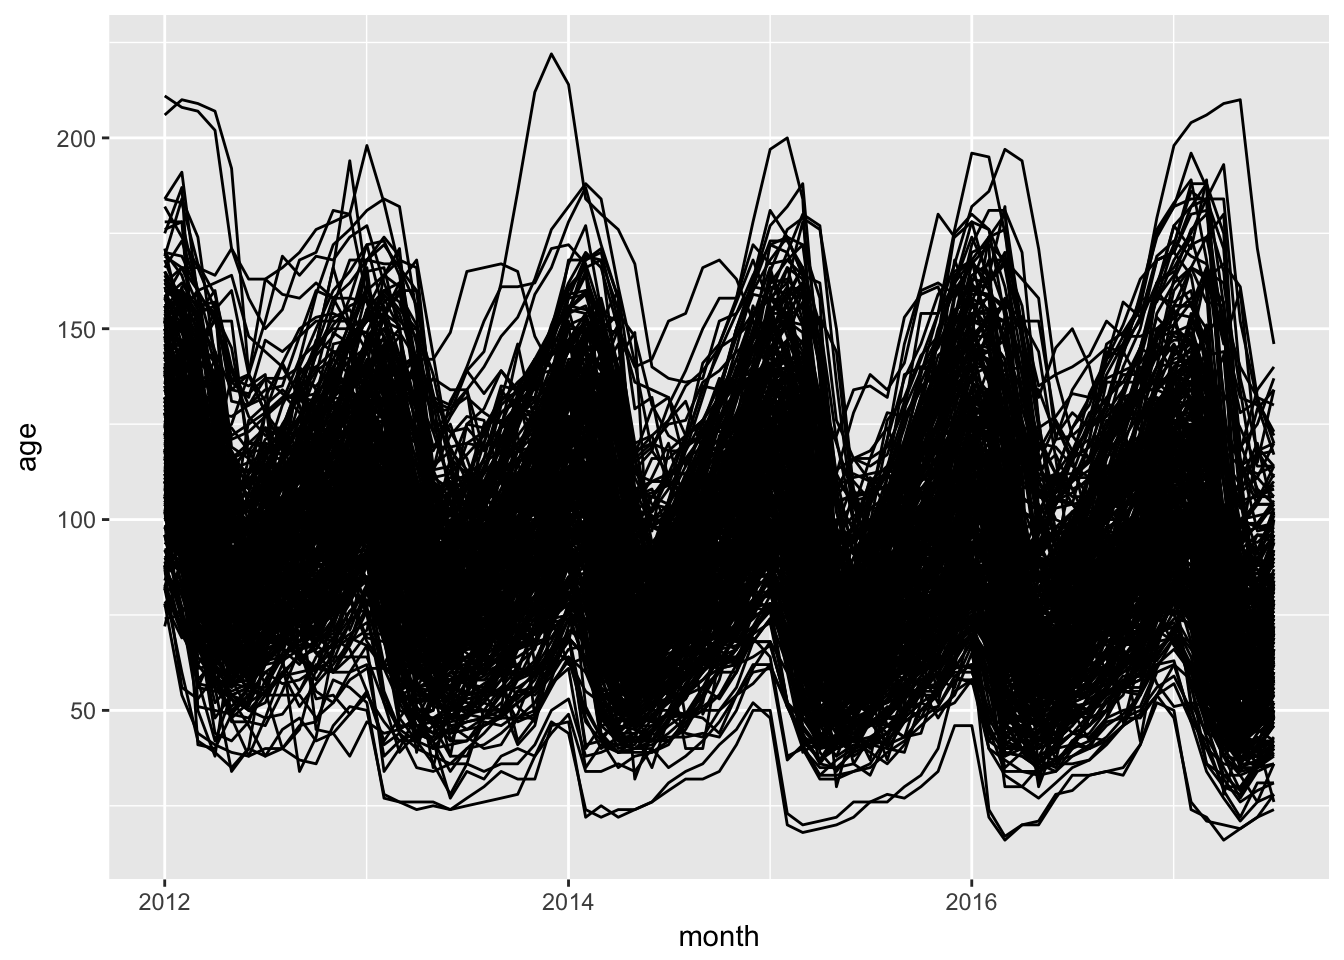
\includegraphics{jonpage-r-course_files/figure-latex/unnamed-chunk-5-1.pdf}

\section{gganimate}\label{gganimate}

The \texttt{gganimate} package lets us animate the above chart. If you
want to be able to save animations as an mp4, you will need install
\texttt{ffmpeg} (\url{https://www.ffmpeg.org/download.html}). You can
install \texttt{gganimate} with \texttt{devtools}:

\begin{verbatim}
devtools::install_github("dgrtwo/gganimate")
\end{verbatim}

\begin{Shaded}
\begin{Highlighting}[]
\KeywordTok{library}\NormalTok{(gganimate)}
\NormalTok{f <-}\StringTok{ }\KeywordTok{ggplot}\NormalTok{(wind, }\KeywordTok{aes}\NormalTok{(lon, lat, }\DataTypeTok{angle =} \NormalTok{angle, }\DataTypeTok{radius =} \NormalTok{radius, }\DataTypeTok{alpha =} \NormalTok{radius, }\DataTypeTok{color =} \NormalTok{angle, }\DataTypeTok{frame =} \NormalTok{time)) +}
\StringTok{  }\KeywordTok{geom_spoke}\NormalTok{() +}
\StringTok{  }\KeywordTok{scale_color_gradient2}\NormalTok{(}\DataTypeTok{low =} \StringTok{"#132B43"}\NormalTok{, }\DataTypeTok{mid =} \StringTok{"#56B1F7"}\NormalTok{, }\DataTypeTok{high =} \StringTok{"#132B43"}\NormalTok{)}
\KeywordTok{gganimate}\NormalTok{(f)}
\end{Highlighting}
\end{Shaded}

\chapter{geom\_area and geom\_ribbon}\label{area-and-ribbons}

\part{Topics}\label{part-topics}

\chapter*{Anscombe's Quartet}\label{anscombe}
\addcontentsline{toc}{chapter}{Anscombe's Quartet}

\chapter*{How to Judge Visualizations}\label{trifecta}
\addcontentsline{toc}{chapter}{How to Judge Visualizations}

\bibliography{packages.bib,book.bib}


\end{document}
